\documentclass[11pt]{ekblite}
\newcommand\mtop{1in}
\newcommand\mbottom{1in}
\newcommand\mleft{1.2in}
\newcommand\mright{1.2in}
\usepackage[top=\mtop, bottom=\mbottom, left=\mleft, right=\mright]{geometry}

\newcommand{\comment}[1]{}
\newcommand\aaron[1]{\textcolor{red}{#1}}
\newcommand{\seay}[1]{\textcolor{blue}{#1}}
\hypersetup{ 	
pdfsubject = {Mathematics},
pdftitle = {fractal dimension},
pdfauthor = {Max Seay and Aaron Huntley}
}

\begin{document}

\title{Exploring fractal dimension\\
DRP spring 2025}
\maketitle
\begin{center}
Maxwell Seay and Aaron Huntley\\
\today
\end{center}

\tableofcontents

\newpage

\section{Preface}
This was written by Max Seay of CWRU with direction from PhD student Aaron Huntley, as part of the Directed Reading Program in Spring 2025. As of writing, it has not been proofread.

\newpage
\section{Introduction}
The goal is to find how to compute \textit{dimensionality}. I already know the \textit{dimensionality} of some things. I know the dimension of a point is 0, the dimension of a line is 1, the dimension of a square is 2, etc. But how is it calculated for some arbitrary object? In this case, by object, I mean:
\\[0.2in]A finite or infinite \textit{compact} set of points $x$, where $x \subset \R^n$.
\\[0.2in] \cite{edgar} applies Hausdorff measure (and probably other things) to compact sets in $\R^n$ only. From what I've read the other sources make the same assumption.
\\[0.2in]Below are common examples of objects and their dimension.
\begin{example}[Point]
	A point is a single element of a metric space $X$. For example, any single number is a point in the metric space $\R$ (the real number line.) 
	\[p_1 = \{1\}\]
	\[p_2 = \{2\}\]
	\[p_3 = \{3\}\]
	\[p_4 = \{\pi\}\]
	The above $p_1$, $p_2$, $p_3$, $p_4$ are examples of points inside the metric space $\R$. This object is known to have dimension 0. The set contains only one item, only one number.
\end{example}
\begin{example}[Unit line segment]
	The unit line segment is a subset of $\R$, the real number line, defined as the set 
	\[\{x : 0 \le x \le 1\}\]
	In other words, the unit line segment is a set containing every real number between and including 0 and 1.
	\\[0.2in]This object is known to have dimension 1. The set contains an uncountably infinite amount of real numbers.
\end{example}
\begin{example}[Unit square]
	The unit square is a subset of $\R^2$, the Euclidean plane, defined as the set of points
	\[\{(x,y) : 0 \le x \le 1, 0 \le y \le 1\}\]
	In other words, the unit square is a set containing every real number inside a square.
	\\[0.2in]This object is known to have dimension 2. The set contains an uncountably infinite amount of real numbers.
\end{example}
\begin{example}[Finite sets]
	A point is a 0-dimensional element of a metric space. And the union of two points is also 0-dimensional.
	\\[0.2in]Any finite set of points has dimension 0. More generally, any finite union of $m$-dimensional sets has dimension $m$. (Union is used to combine two sets into one bigger set. $\{a\} \cup \{b\} = \{a,b\}$).
	\\[0.2in]The focus for this however is on weird sets. Sets that are made of $m$-dimensional objects but which are $n$-dimensional, where $m < n$. Somehow a set that breaks from one dimension into another. Already it can be seen one requirement of this strangeness:
	\\[0.2in]The set must contain an infinite number of elements.
	\\[0.2in]Finite sets are too well behaved. By the upcoming definitions of dimension, a finite union of objects with dimension $m$ will also still have dimension $m$. 
\end{example}



\newpage
\section{How to measure the real numbers}
\newpage
\section{Notion of dimension: Minkowski–Bouligand or box-counting dimension}
I would like to know how to estimate the dimension of arbitrary objects. First I will look at simple examples to find out more about the notion of dimension.
\begin{example}[Line segment]
	I know what a line segment is. I also know every line segment is 1 dimensional.
	\\[0.2in]I take an approximation. I will cover a line segment with boxes. Each box has diameter (or radius) $r$. (To me it doesn't matter much since the difference between radius and diameter is always just a factor of 2.)
	\\[0.2in]Take the line segment to be the interval $[0,1]$. If $r = 1$, then I need only 1 box to cover the line segment.
	\\[0.2in]If $r = \sfrac{1}{2}$, I will need at least 2 boxes.
	\\[0.2in]If $r = \sfrac{1}{3}$, I will need at least 3 boxes.
	\\[0.2in]If $r = \sfrac{1}{n}$, I will need at least $n$ boxes to cover the line segment.
	\\[0.2in]I will define a function that takes in a radius, $r$, and outputs the least number of boxes of radius $r$ needed to cover the line segment. From the above examples it can be seen that this function is:
	\[\mathcal{N}(r) = \frac{1}{r}\]
	Another idea to think on. How to double the \textit{length} of the line segment? To double the length of the line segment, copy and paste it once, and append the copy onto the end of the original. 
	\\[0.2in]So in other words, to double the length of the line segment, add 1, (or $2^1 - 1$ you could say,) extra copy.
\end{example}
\begin{example}[Square]
	I know what a square is. I also know every square is 2 dimensional.
	\\[0.2in]I take an approximation. I will cover a square with boxes. Each box has diameter (or radius) $r$.
	\\[0.2in]Take the square to be the unit square, $[0,1] \times [0,1]$. If $r = 1$, then I need only 1 box to cover the square. (The box and square are the same.)
	\\[0.2in]If $r = \sfrac{1}{2}$, I will need at least 4 boxes.
	\\[0.2in]If $r = \sfrac{1}{3}$, I will need at least 9 boxes.
	\\[0.2in]If $r = \sfrac{1}{n}$, I will need at least $n^2$ boxes to cover the unit square.
	\\[0.2in]I will define a function that takes in a radius, $r$, and outputs the least number of boxes of radius $r$ needed to cover the square. From the above examples it can be seen that this function is:
	\[\mathcal{N}(r) = \frac{1}{r^2}\]
	Now how to double the \textit{area} of the square? To double the area of the square, copy and paste it three times, and append the copies to three sides of the original. 
	\\[0.2in]So in other words, to double the area of the square, add 3, (or $2^2 - 1$ you could say,) extra copies.
\end{example}
So for the line segment we have that the number of squares of radius $r$ needed to cover it as
\[\mathcal{N}(r) = \frac{1}{r}\]
And for the square we have that the number of squares of radius $r$ needed to cover it as
\[\mathcal{N}(r) = \frac{1}{r^2}\]
From these couple examples it seems that, in general
\[\mathcal{N}(r) = c \left(\frac{1}{r}\right)^d\]
Where $c$ is a constant. It seems that it would be appropriate to call the $d$ in this expression the dimension. This function $\mathcal{N}(r)$ is called a power law since $\sfrac{1}{r}$ is always raised to some power. \cite{falconer2}

\newpage
\section{Notion of Dimension: Hausdorff measure and dimension}
\newpage
\section{Cantor Set}
	Let $\mathcal{C}$ be the Cantor Set.
	\begin{definition}[Cantor Set]
        $\mathcal{C}$ can be described as an intersection of an infinite sequence of sets. The sequence of sets, $\{\mathcal{C}_i\}_{i=0}^{\infty}$, is defined recursively. For example, the first three are:
		\[C_0 = [0,1]\]
		\[C_1 = \left[0,\sfrac{1}{3}  \right] \cup \left[ \sfrac{2}{3},1\right]\]
		\[C_2 = \left[0,\sfrac{1}{9}  \right] \cup \left[ \sfrac{2}{9},\sfrac{3}{9} \right] \cup \left[\sfrac{6}{9},\sfrac{7}{9}\right] \cup \left[ \sfrac{8}{9},1\right]\]
		\[C_3 = \left[0,\sfrac{1}{27}  \right] \cup \left[\sfrac{2}{27},\sfrac{3}{27}  \right] \cup \left[\sfrac{6}{27},\sfrac{7}{27}  \right] \cup \left[\sfrac{8}{27},\sfrac{9}{27}  \right] \cup \left[\sfrac{18}{27},\sfrac{19}{27}  \right] \cup \left[\sfrac{20}{27},\sfrac{21}{27}  \right] \cup \left[\sfrac{24}{27},\sfrac{25}{27}  \right] \cup \left[\sfrac{26}{27},1  \right]\]
		\\
		And the recursive definition for a set $\mathcal{C}_i$ is:
		\[\mathcal{C}_i = \frac{1}{3} \mathcal{C}_{i-1} \cup \frac{2}{3} + \frac{1}{3} \mathcal{C}_{i-1}\]
		Or an alternate (non-recursive) definition for a set $\mathcal{C}_i$ is:
		\[\mathcal{C}_i = \bigcup_{j=0}^{i-1} \frac{2j}{3^{i-1}} + \left[j\frac{1}{3^i}, (j+1)\frac{1}{3^i}\right] \cup \left[(j+2)\frac{1}{3^i}, (j+3)\frac{1}{3^i}\right]\]
		(idk I just came up with this. I think it works.)
	\end{definition}
	\begin{corollary}
		$\mathcal{C}_i \ne \mathcal{C}$ for all $i \in \mathbb{N}$. No set in the sequence $\{\mathcal{C}_i\}$ is the Cantor Set, however the further you go (the larger the $i$), the ``closer'' $\mathcal{C}_i$ becomes $\mathcal{C}$. 
	\end{corollary}
	\begin{corollary}
		If $x \notin [0,1]$, then $x \notin \mathcal{C}$.
	\end{corollary}
	\begin{corollary}
		The Cantor Set is non-empty.
	\end{corollary}
	\begin{proof}Consider the point 0.
	\\[0.2in]$0 \in [0,1]$ so $0 \in \mathcal{C}_0$.
	\\[0.2in]Now make the assumption that $0 \in \mathcal{C}_k$.
	\\[0.2in]And since $\frac{1}{3} \cdot 0 = 0$ it must be true that
	\[0 \in \frac{1}{3} \cdot \mathcal{C}_k\] 
	\\[0.2in]Note that by definition we have that
	\[\mathcal{C}_{k+1} = \frac{1}{3} \mathcal{C}_{k} \cup \frac{2}{3} + \frac{1}{3} \mathcal{C}_{k}\]
	Well since $0 \in \frac{1}{3} \cdot \mathcal{C}_k$ it must be true that
	\[0 \in \frac{1}{3} \mathcal{C}_{k} \cup \frac{2}{3} + \frac{1}{3} \mathcal{C}_{k}\]
	or
	\[0 \in \mathcal{C}_{k+1}\]
	So by induction we have that
	\[0 \in \mathcal{C}\]
	Thus $\mathcal{C}$ is non-empty.
	\end{proof}
	\begin{corollary}
		The Cantor Set is a proper subset of $[0,1]$.
	\end{corollary}
	\begin{corollary}
		$\mathcal{C}_{i}$ is always a covering of $\mathcal{C}_{i+1}$ and also always a covering of $\mathcal{C}$.
	\end{corollary}
	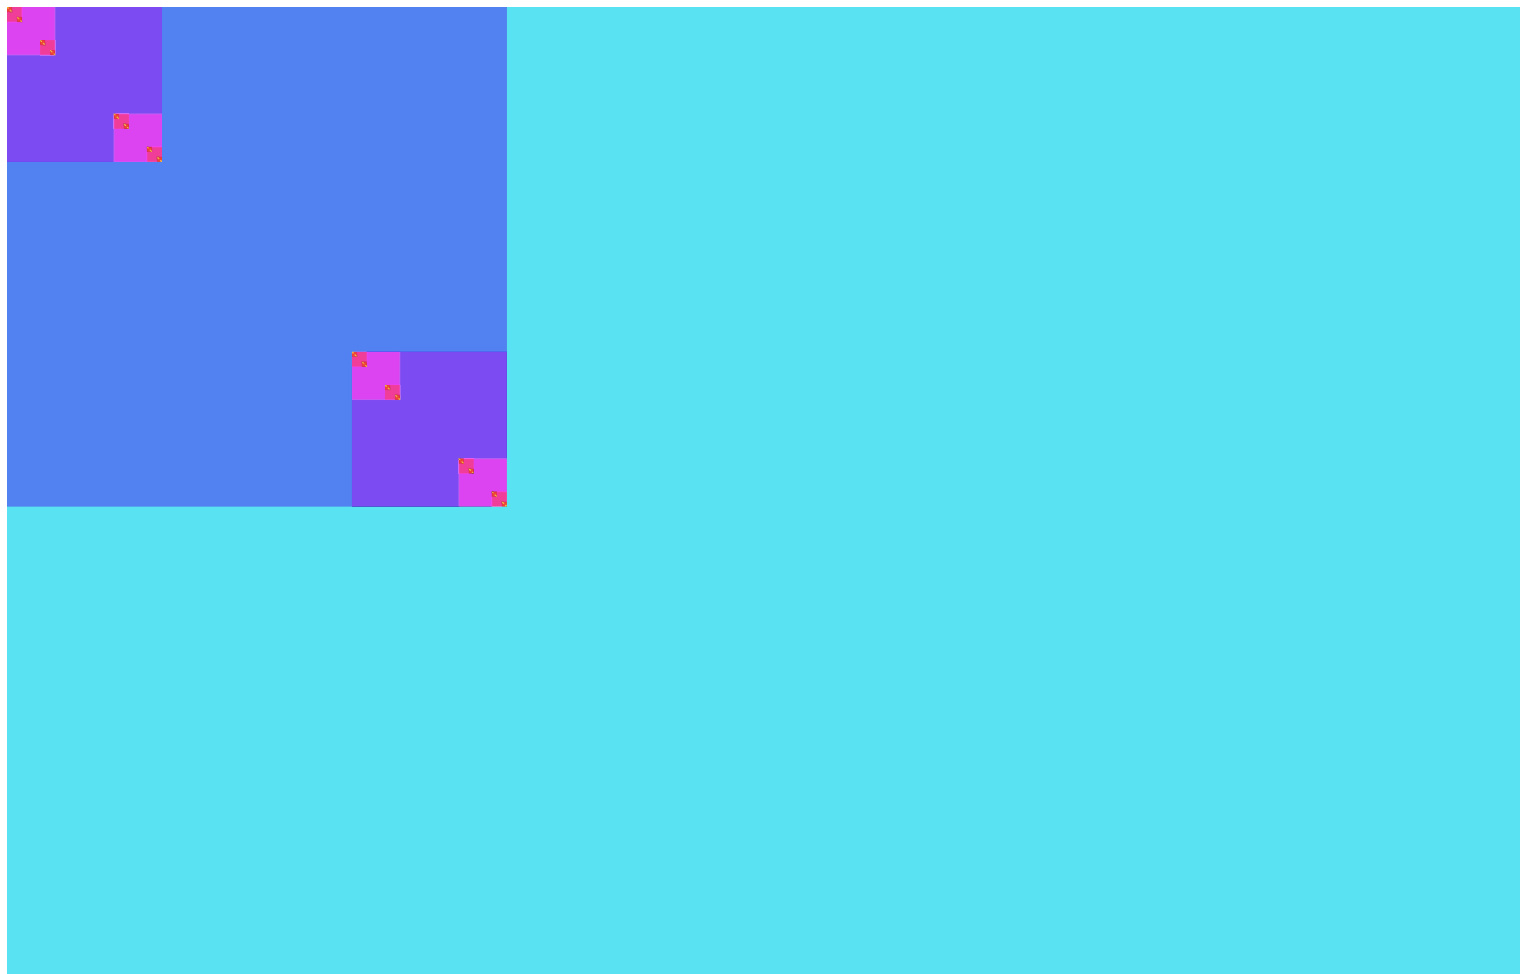
\includegraphics[scale=0.2]{img/c1.jpg}
	\\Cantor Set visualized in 2D with 10 iterations. For each interval $[a,b]$ of the set, there is a colored box positioned at $(a,a)$ with size $(3^{-k}, 3^{-k})$, where $k$ is the iteration. 
	\\[0.2in]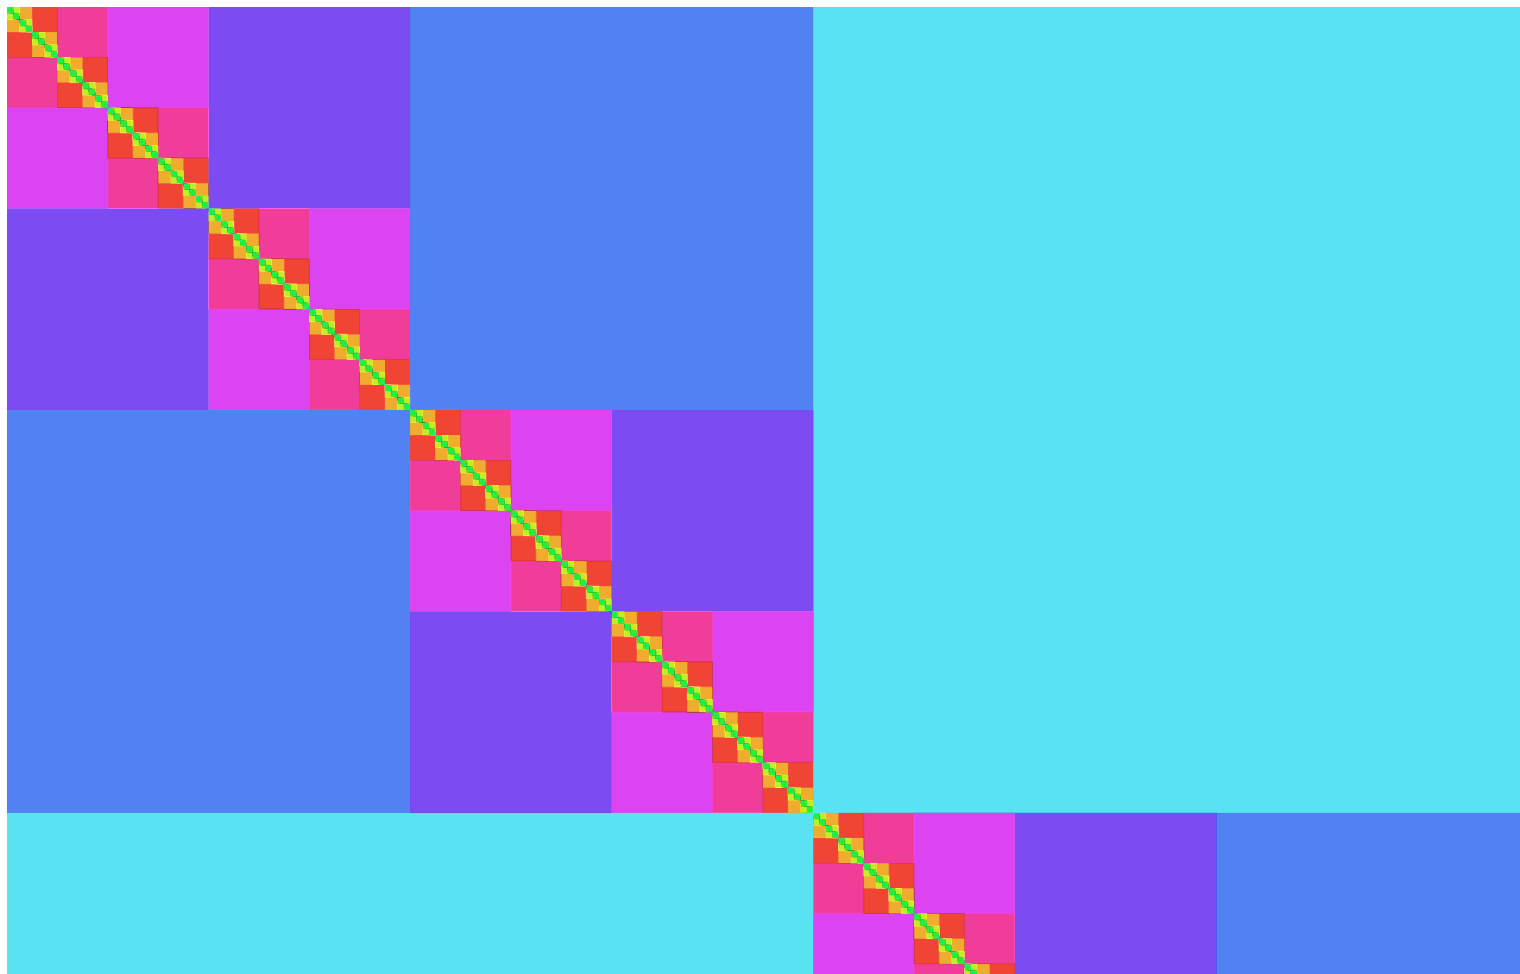
\includegraphics[scale=0.2]{img/c2.jpg}
	\\A set visualized in 2D with 10 iterations constructed the same way as the Cantor Set. However the $\frac{1}{3}$ in the Cantor Set definition is replaced with $\frac{1}{2}$ instead. 
	\\[0.2in]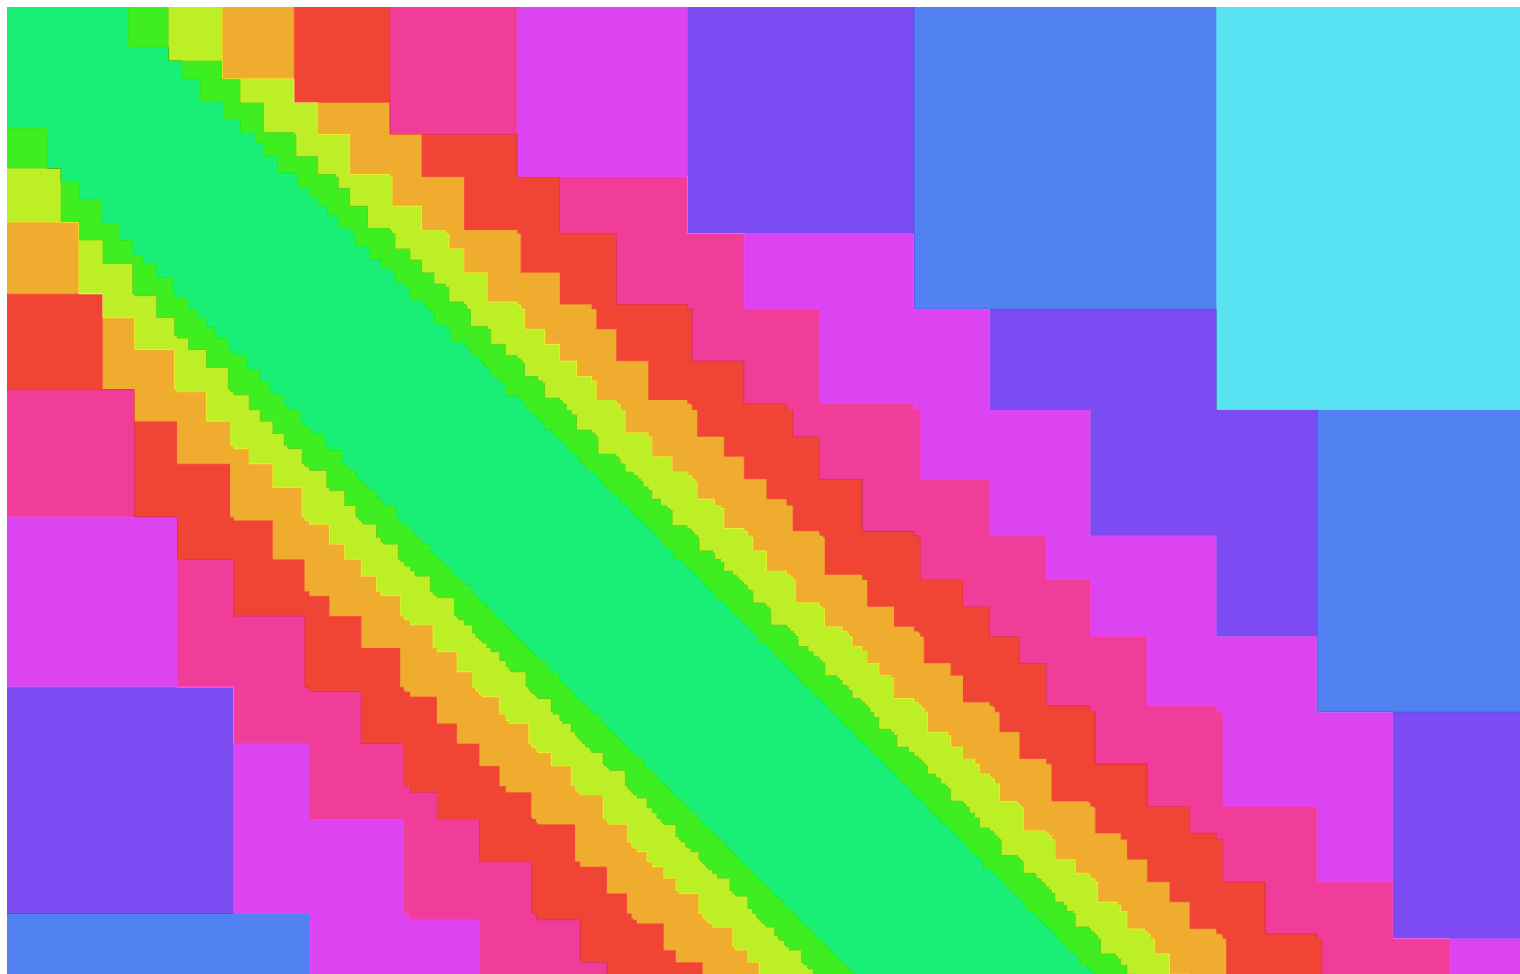
\includegraphics[scale=0.2]{img/c3.jpg}
	\\A set visualized in 2D with 10 iterations constructed the same way as the Cantor Set. However the $\frac{1}{3}$ in the Cantor Set definition is replaced with $\frac{3}{4}$ instead. 
	\\[0.2in]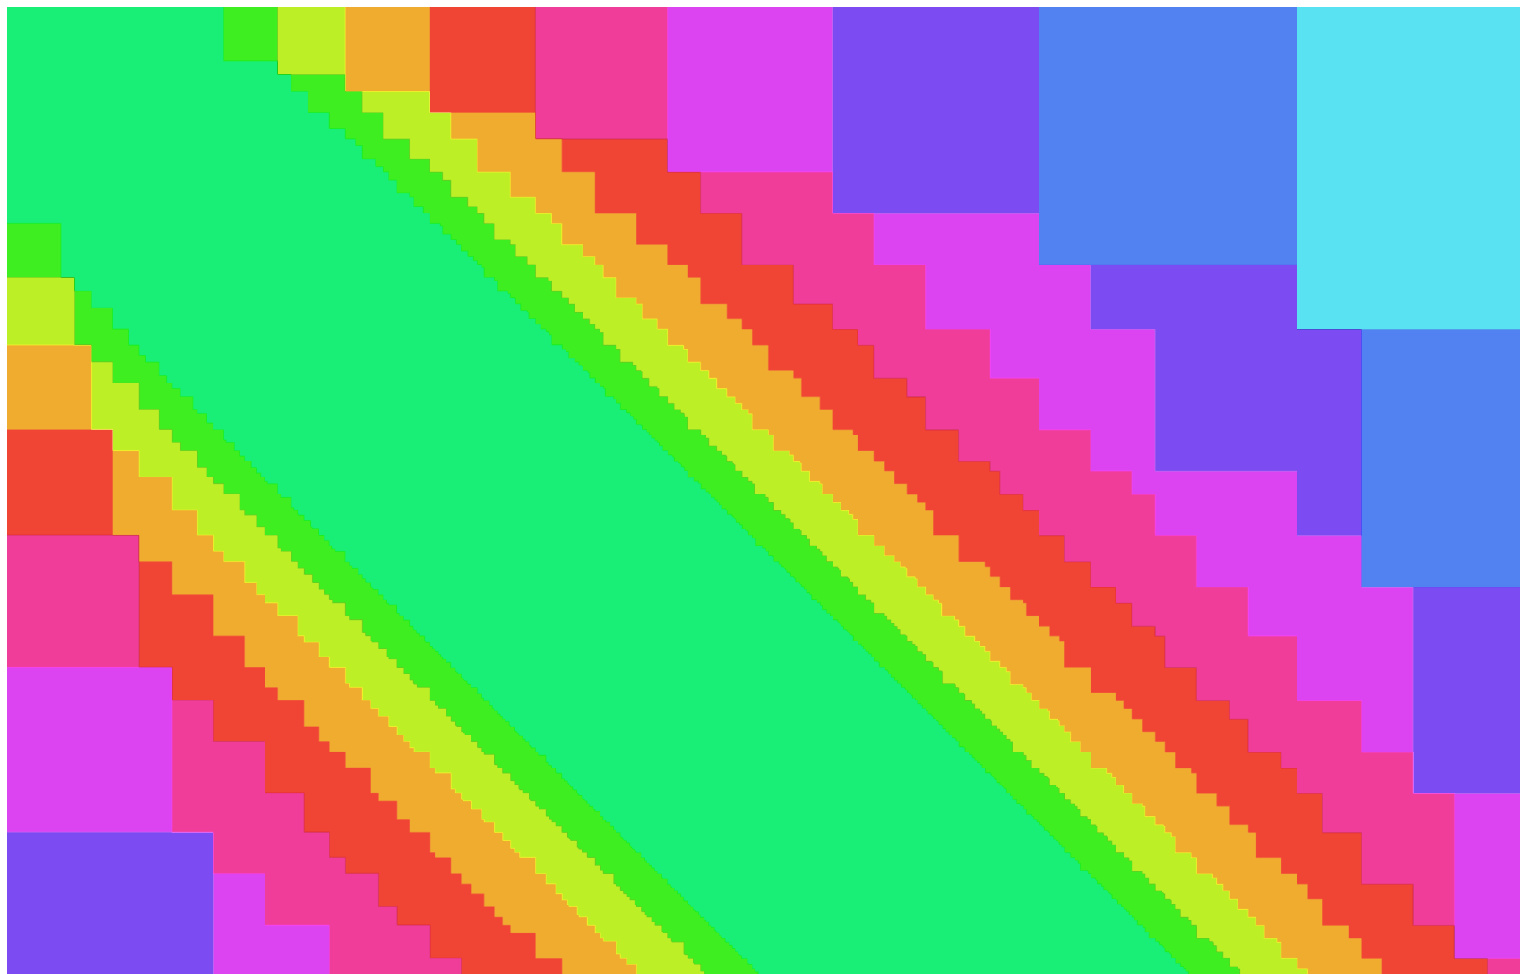
\includegraphics[scale=0.2]{img/c4.jpg}
	\\A set visualized in 2D with 10 iterations constructed the same way as the Cantor Set. However the $\frac{1}{3}$ in the Cantor Set definition is replaced with $\frac{4}{5}$ instead. 
\newpage
\section{Dragon}

\newpage
\bibliography{citations}

\end{document}
